\section{Visão Geral do \textit{Pipeline} de Processamento}
\label{cap:7.2}

O \textit{pipeline} de processamento proposto para o desenvolvimento das soluções baseadas em aprendizado de máquina está representado, em alto nível, pela Figura \ref{fig:25}, sendo notória a existência de quatro fases de execução. Cada uma dessas fases é descrita nas subseções a seguir, mas todas elas compartilham das mesmas configurações gerais. O compartilhamento dessas configurações permite que as quatro fases mantenham uma sincronia em relação a variáveis como as sequências de vídeo a serem utilizadas, núcleos de processamento autorizados para uso, arquivos a serem substituídos nos softwares de referência, identificações e meios de compilação desses softwares, lista de configurações dos hiperparâmetros do algoritmo de aprendizado de máquina, entre outros valores. Essa centralização de configurações facilita a realização de modificações rápidas nos experimentos, garantindo uma maior agilidade e confiabilidade no \textit{pipeline}.

\begin{figure}
    \centering
    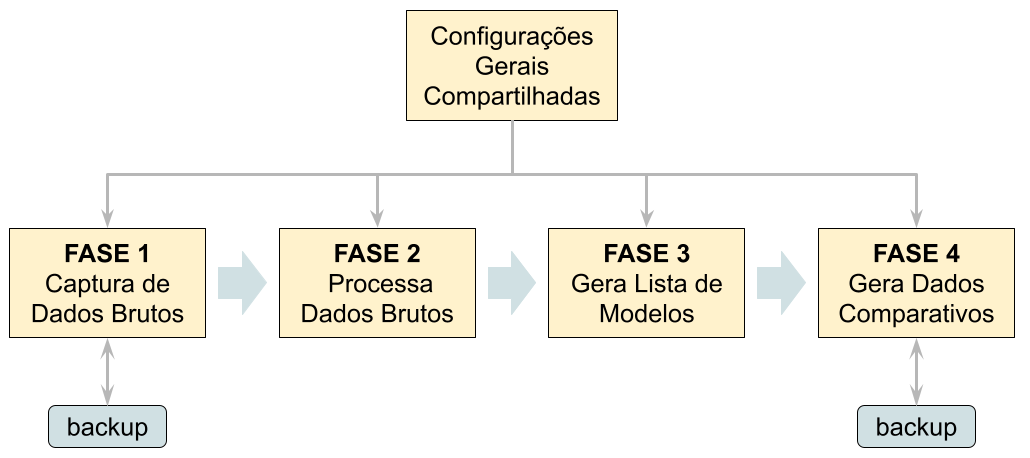
\includegraphics[width=\textwidth]{FIGURES/fig_25.png}
    \caption{Representação em alto nível do fluxo de execução do \textit{pipeline} de processamento. Fonte: Elaborada pelo autor.}
    \label{fig:25}
\end{figure}

Após a configuração geral do experimento e dos softwares, conforme descrito na seção \ref{cap:4.2}, o \textit{pipeline} automatiza a execução de todas as quatro fases. Nas Fases 1 e 4, um sistema de backup auxilia a retomada dos experimentos em caso de interrupção. A Fase 3 é responsável pela seleção do melhor modelo de aprendizado de máquina treinado com os dados gerados da Fase 2.

O algoritmo implementado no transcodificador rápido de VP9-para-AV1, e que será adaptado para os demais formatos considerados neste capítulo, será utilizado nas Fases 1, 2 e 4. Esse algoritmo será descrito com detalhes na seção \ref{cap:7.4}. Enquanto a seleção do melhor modelo de aprendizado de máquina (Fase 3) é descrita na seção \ref{cap:7.3}. O código-fonte do \textit{pipeline} proposto está disponível em \citet{bib:prototipotese}.

\subsection{Fase 1: Captura de Dados Brutos}
\label{cap:7.2.1}

É responsabilidade desta fase a captura dos dados brutos para treinamento e teste dos modelos de aprendizado de máquina. Os vídeos codificados no antigo formato são decodificados, gerando dois arquivos: o vídeo decodificado e os dados extraídos durante a decodificação. A partir do vídeo decodificado, a transcodificação é concluída com uma recodificação do conteúdo no novo formato, sem qualquer processo de aceleração, exportando um conjunto de dados. O fluxo de execução da Fase 1 é demonstrado na Figura \ref{fig:26}. Em todas as soluções apresentadas neste capítulo, o codificador utilizado foi o software \textit{libaom} do AV1. De forma geral, esta fase é responsável por:

\begin{enumerate}[1.]
    \item Decodificar o \textit{bitstream} pertencente ao conjunto de treinamento e de teste, que foi codificado em um formato pré-definido;

    \item Exportar informações provenientes do decodificador;

    \item Recodificar o vídeo decodificado para o novo formato, utilizando parâmetros de quantização pré-definidos;

    \item Exportar informações provenientes do codificador.
\end{enumerate}

\begin{figure}
    \centering
    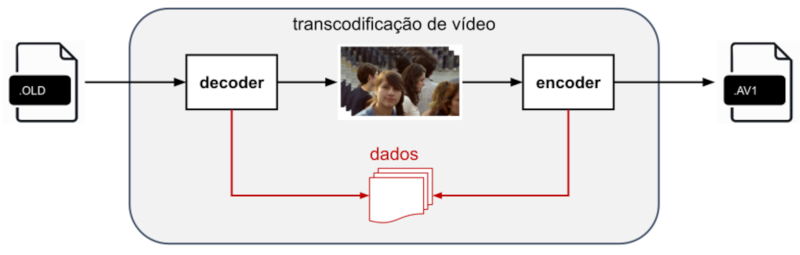
\includegraphics[width=0.85\textwidth]{FIGURES/fig_26.png}
    \caption{Representação da transcodificação realizada na Fase 1. Fonte: Elaborada pelo autor.}
    \label{fig:26}
\end{figure}


\subsection{Fase 2: Processamento de Dados Brutos}
\label{cap:7.2.2}

É responsabilidade desta fase o processamento dos dados brutos extraídos na primeira fase, de forma a gerar amostras passíveis de realizar corretamente o treinamento e o teste dos modelos treinados por aprendizado de máquina. Apesar de o processamento geral dos dados feito aqui também ser executado na fase 4, há uma significativa diferença entre ambos: na fase 4, toda a execução é feita internamente ao software codificador, enquanto aqui o processamento é executado externamente. Além disto, nesta segunda fase, também são processadas as decisões realizadas pelo codificador, a separação de conjuntos de dados em subconjuntos para cada modelo e o balanceamento de dados. Mais informações sobre os subconjuntos serão apresentadas na seção \ref{cap:7.3}. De forma geral, esta fase é responsável por:

\begin{enumerate}[1.]
    \item Unificar os dados extraídos na Fase 1, sob diferentes níveis de quantização;

    \item Remover elementos inválidos, existentes no conjunto de dados brutos;

    \item Dividir o conjunto de dados em subconjuntos de dados;

    \item Identificar os rótulos (decisões) para cada subconjunto;

    \item Balancear os dados;

    \item Exportar os dados balanceados em arquivos para treinamento e teste de cada modelo, conforme definido na seção \ref{cap:7.3}.
\end{enumerate}

Na responsabilidade 2, listada acima, acontece a remoção de elementos inválidos, pois, como veremos na seção \ref{cap:7.4}, regiões de borda do vídeo não são visíveis na imagem e, portanto, não podem gerar amostras passíveis de serem preditas pelo modelo de aprendizado de máquina.

O rótulo utilizado na proposta de transcodificador rápido deste capítulo é o subparticionamento do bloco atual em processamento, como melhor será abordado na seção \ref{cap:7.4}. Portanto, a identificação do rótulo (responsabilidade 4) é obtida com a observação das estruturas de particionamento existentes: caso o atual nível de profundidade seja subparticionado, então o rótulo é positivo (particiona), caso contrário, negativo (não particiona).

Como vimos no capítulo \ref{cap:5}, existe um desbalanceamento de ocorrência de particionamento de acordo com o nível de profundidade da árvore. Portanto, o balanceamento das amostras válidas é necessário para possibilitar o treinamento de modelos de forma mais correta. Nas soluções apresentadas nesta tese, optamos por balancear os dados em 50\%-50\%, ou seja, manter aproximadamente o mesmo número de exemplos com o rótulo positivo e com o rótulo negativo para cada subconjunto de amostras criado.

Existem duas principais técnicas de balanceamento de dados \cite{bib:livroRaschka}: \textbf{\textit{undersampling}}, onde remove-se amostras do rótulo majoritário e \textbf{\textit{oversampling}}, onde aumenta-se a representatividade dos dados do rótulo minoritário. Apesar de ambas apresentarem prós e contras, em geral as duas ocasionam um aumento no viés dos dados, seja por remover amostras importantes no treinamento, seja por ocasionar um sobreajuste dos dados, ou seja, gerar um modelo inviável para lidar com novos dados. Embora haja uma vasta literatura sobre como lidar com dados desbalanceados, como pode ser visto em \citet{bib:livroimbalanced}, não existe uma forma consolidada para automatizar o processo de análise de balanceamento de dados. Ou seja, ainda não é possível excluir o fator humano no processo de escolha do melhor balanceamento a ser aplicado nos dados, pois há a necessidade de avaliar os resultados e contexto de aplicação do modelo preditivo. Logo, optamos pela técnica de \textit{undersampling} através da remoção aleatória de amostras do conjunto majoritário. Para garantir a adaptabilidade desse processo, uma semente geradora de números aleatórios de valor 42 foi utilizada. 

\subsection{Fase 3: Geração de Lista de Modelos Preditivos}
\label{cap:7.2.3}

É responsabilidade desta fase o treinamento e o teste de todos os modelos preditivos gerados por algoritmos de aprendizado de máquina, além da seleção do melhor modelo para ser utilizado na fase de predição dos resultados. É com a combinação das configurações dos hiperparâmetros a serem utilizados (vide Tabela \ref{tab:XVIII}) que se obtém a lista completa de candidatos a serem treinados e testados. Neste processo, consideramos um universo de 9.526.572 candidatos de modelos de aprendizado de máquina para o algoritmo de árvore de decisão CART. Apesar disso, a modificação dos candidatos ou do próprio algoritmo de aprendizado de máquina é simples e não altera os demais fluxos automatizados do \textit{pipeline} de processamento.

É na seção \ref{cap:7.3} que iremos abordar com maiores detalhes os modelos treinados, contudo, para melhor compreensão desta subseção, se faz necessário a apresentação de alguns termos e informações. Na proposta de transcodificador rápido com uso de modelos preditivos, realizado nesta tese, iremos utilizar um grupo de modelos preditivos que trabalharão em conjunto, cada um responsável por predizer o rótulo sob condições específicas. Mais precisamente, há um modelo treinado para cada nível de profundidade da árvore do AV1, sob diferentes níveis de quantização. Dessa forma, como descreveremos melhor na seção \ref{cap:7.3}, há 12 modelos nesse conjunto, todos eles treinados sob o mesmo candidato de combinação de hiperparâmetros.

Dessa forma, a escolha pelo melhor candidato é feita através de uma competição iterativa entre os candidatos. Partindo-se de uma quantidade limitada e pequena de amostras, cada iteração dobra essa quantidade de amostras e, ao mesmo tempo, reduz pela metade o número de candidatos. Com isso, avaliamos todos os candidatos sob as mesmas condições e, após alguns ciclos iterativos e aceitando algum nível de incerteza, chega-se a ao melhor candidato. De forma geral, esta fase é responsável por:

\begin{enumerate}[1.]
    \item Gerar uma lista de candidatos a serem avaliados, com base no produto das variações dos hiperparâmetros;

    \item Avaliar todos os candidatos para cada um dos 12 modelos do grupo de modelos. De cada modelo treinado, selecionar os melhores 20 candidatos;

    \item Treinar o grupo de modelos com cada um dos candidatos de hiperparâmetros, com o conjunto completos de dados;

    \item Testar todos os modelos treinados com o conjunto de dados de teste;

    \item Reprovar modelos cujo AUC for inferior ao limite mínimo estabelecido na seção \ref{cap:7.3};

    \item Remover candidatos de hiperparâmetros que não tiverem todos os modelos aprovados;

    \item Calcular média de \textit{F1-Score} para todos os candidatos aprovados e ordená-los em ordem decrescente;

    \item Indicar para o restante do fluxo do \textit{pipeline} qual foi o candidato vencedor.
\end{enumerate}

\subsection{Fase 4: Geração de Dados Comparativos}
\label{cap:7.2.4}

É responsabilidade desta fase a geração dos dados comparativos entre a transcodificação rápida com uso dos modelos preditivos gerados por algoritmo de aprendizado de máquina, treinados com o candidato vencedor da Fase 3, em relação à transcodificação original. Nesta fase, são executadas as duas transcodificações e, consequentemente, sendo a fase mais custosa do \textit{pipeline}. De forma geral, esta fase é responsável por:

\begin{enumerate}[1.]
    \item Decodificar o \textit{bitstream} do conjunto de predição, que foi previamente codificado em algum formato pré-definido;

    \item Exportar informações provenientes do decodificador;

    \item Recodificar o vídeo decodificado para o novo formato, utilizando os níveis de quantização pré-definidos, utilizando a transcodificação original;

    \item Recodificar o vídeo decodificado para o novo formato, utilizando os níveis de quantização pré-definidos, utilizando a nossa proposta de transcodificador rápido;

    \item Exportar dados de transcodificação para permitir uma comparação objetiva.
\end{enumerate}
